\documentclass[12pt, twoside]{article}
\usepackage[francais]{babel}
\usepackage[T1]{fontenc}
\usepackage[latin1]{inputenc}
\usepackage[left=7mm, right=7mm, top=7mm, bottom=7mm]{geometry}
\usepackage{float}
\usepackage{graphicx}
\usepackage{array}
\usepackage{multirow}
\usepackage{amsmath,amssymb,mathrsfs}
\usepackage{soul}
\usepackage{textcomp}
\usepackage{eurosym}
 \usepackage{variations}
\usepackage{tabvar}

\begin{document}


\section*{\center{Aide individualis�e: Fonctions de r�f�rence}}


\begin{enumerate}
  \item Ecrire la d�finition de fonction croissante et illustrer la d�finition
  par un sch�ma.


  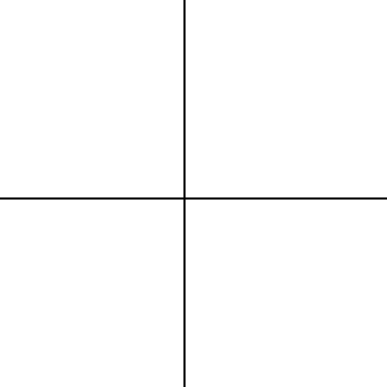
\includegraphics[width=20mm]{images/repere.png}

 
  
  
 \item Ecrire la d�finition de fonction croissante et illustrer la d�finition
  par un sch�ma.  
  
  
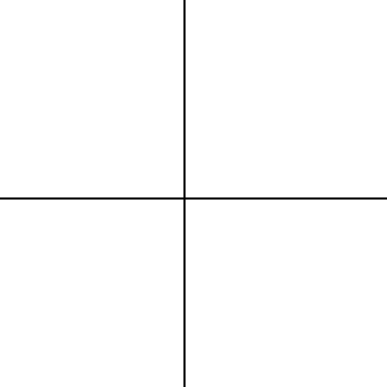
\includegraphics[width=20mm]{images/repere.png}
   
     
   \item
 \begin{enumerate}
       \item Tracer la courbe repr�sentative de la fonction carr� (sch�ma).
       \item Dresser le tableau de variation de la fonction carr�.
      \item D�crire le sens de variations de la fonction carr� avec une phrase. 
  \end{enumerate}  
   
   \enskip
   
   \fbox{ \begin{minipage}{185mm}
          Une propri�t� de variation s'exprime par une
   phrase du type: ``la fonction \ldots est \ldots sur l'intervalle \ldots''.
          \end{minipage}}
 
   \bigskip
   
   
   \bigskip
   
   \bigskip
   
   \item 
 \begin{enumerate}
       \item Tracer la courbe repr�sentative de la fonction inverse (sch�ma).
       \item Donner le domaine de d�finition de la fonction inverse.
       \item Dresser le tableau de variation de la fonction inverse.
      \item D�crire le sens de variations de la fonction inverse avec une
      phrase.
 \end{enumerate}   
 
 \bigskip
 
 \bigskip
 

 
\end{enumerate}

\subsection*{Exercice}

\begin{enumerate}
  \item On consid�re la fonction $f$ d�finie sur $\mathbb{R}$ par:
  $f(x)=(x-1)^2-2$.
  \begin{enumerate}
    \item Compl�ter et expliquer chaque �tape du raisonnement suivant:
    

    Soit  $a< b<1$  
    
    
    donc  $a-1$ \ldots \ldots   $b-1$ \ldots \ldots,    \qquad    explication:
    
    donc  $(a-1)^2$  \ldots \ldots $(b-1)^2$,  \qquad  \qquad explication:
    
    donc $(a-1)^2-2$  \ldots \ldots $(b-1)^2-2$,  \quad explication:
    
    \item Quelle propri�t� de $f$ a-t-on d�montr�e?
  \end{enumerate}
  
  \item On consid�re la fonction $g(x)=3+\dfrac{1}{x-2}$ d�finie sur
  $\mathbb{R}$ \textbackslash \{2\}
  
  \begin{enumerate}
    \item Ecrire ou compl�ter puis expliquer chacune des �tapes:
    
    Soit $2<a<b$
    
    
    donc:
    
    \bigskip
    
    \bigskip
    
    
    \bigskip
    
    
    donc: $3+ \dfrac{1}{a-2} \ldots \ldots 3+ \dfrac{1}{b-2}$
    \item Quelle propri�t� de $g$ a-t-on d�montr�e?
  \end{enumerate}
  \item Reprendre le m�me type de raisonnement pour dresser le tableau de
  variation des fonctions: 
  
  $h(x)=(x+2)^2-1$ et $i(x)=2+\dfrac{1}{x-1}$.
  \end{enumerate}

\end{document}
